\documentclass{article}
\title{Exponential function}
\author{Michael Iversen}
\usepackage{graphicx}
\begin{document}
\maketitle
The exponential function is denoted either by $\exp(x)$ or $e^x$. It is defined by the following power series
\begin{equation}
\exp(x) = \sum_{n=0}^\infty \frac{x^n}{n!}.
\end{equation}
The exponential function has several properties worth noting. First, it satisfies the exponentiation identity
\begin{equation}
\exp(x + y) = \exp(x) \cdot \exp(y).
\end{equation}
Secondly, it is its own derivative,
\begin{equation}
\frac{\mathrm d}{\mathrm dx} \exp(x) = \exp(x).
\end{equation}
When implementing the exponential function numerically it is efficient to use the following expression
\begin{equation}\label{eq:expression}
\exp(x) = 1 + x \cdot \left( 1 + \frac{x}{2} \left( 1 + \frac{x}{3} \left ( 1 + \ldots \right)\right)\right).
\end{equation}
One may check that the right hand side of the above equation is equivalent to the power series by expanding the expression.
We can check numerically that the above expression works by plotting it along with precalculated values. This plot can be seen in figure \ref{fig:exp}
\begin{figure}
\centering
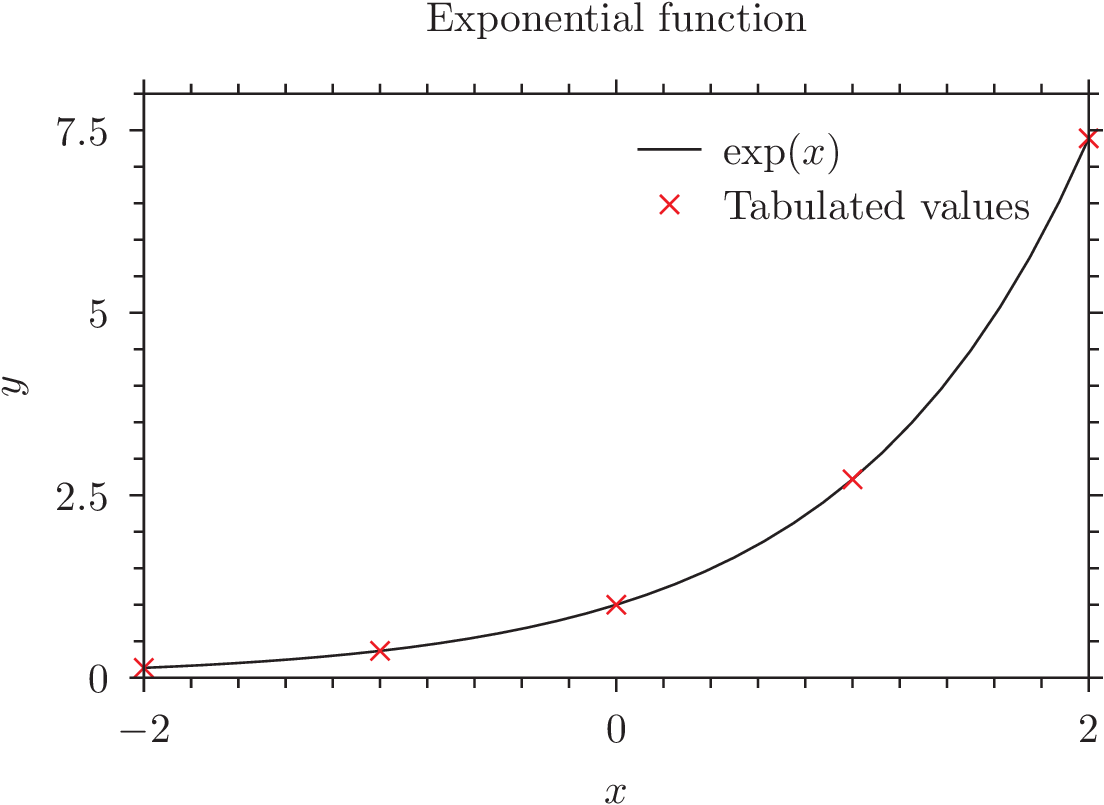
\includegraphics{ex.png}
\caption{The exponential function calculated from equation (\ref{eq:expression}) and tabular values}
\label{fig:exp}
\end{figure}
It is clear from the figure that the expression correctly computes the exponential function. 
Equation (\ref{eq:expression}) is more efficient than the naive power series because it contains fewer mathematical operations.

\end{document}
